\chapter{The Monolithic Quantum Scaling Ceiling}
\label{ch:scaling_ceiling}

\section{Introduction: The Illusion of Monolithic Scalability}
Since the theoretical formulation of the quantum Turing machine by Deutsch in 1985 and the subsequent discovery of polynomial-time quantum algorithms by Shor and Grover, quantum computer science has operated predominantly under a unified, monolithic abstraction. In this classical-analogous paradigm, an ideal quantum processor is conceptualized as an arbitrarily expandable, planar two-dimensional array of physical qubits, governed by localized Hamiltonians and interrogated through synchronized electromagnetic pulses.

For the initial noisy intermediate-scale quantum (NISQ) era—spanning processors from 5 to approximately 100 physical qubits—this monolithic abstraction held firm. Fabrication facilities successfully scaled superconducting transmon processors from the 5-qubit \textit{Bowtie} lattice to the 127-qubit \textit{Eagle} and 433-qubit \textit{Osprey} architectures. In the trapped-ion domain, linear Paul traps reliably sustained one-dimensional ion crystals containing dozens of $^{171}\text{Yb}^+$ ions.

However, as quantum architecture transitions from proof-of-concept NISQ demonstrations toward fault-tolerant quantum computing (FTQC)—where surface codes demand between $10^4$ and $10^7$ physical qubits to support thousands of fault-tolerant logical qubits—the monolithic paradigm encounters unyielding physical, thermodynamic, and topological barriers. 

This chapter establishes the fundamental physical laws and engineering limits that enforce the \textbf{monolithic quantum scaling ceiling}. We demonstrate that building a single, monolithic quantum chip containing millions of high-fidelity physical qubits is not merely an engineering bottleneck, but a thermodynamic impossibility under current and projected cryogenic technologies. Consequently, distributed quantum computing is not an optional architectural preference, but the singular viable pathway toward scalable quantum advantage.

---

\section{The Cryogenic Thermal Bottleneck}

\subsection{Thermodynamics of Dilution Refrigeration}
Superconducting transmons, semiconductor spin qubits, and silicon photonic detectors operate at millikelvin temperatures, typically between $10\text{ mK}$ and $20\text{ mK}$. Maintaining this temperature is essential to suppress thermal excitations across the superconducting energy gap $\Delta \approx 200\,\mu\text{eV}$. At equilibrium, the thermal population of the first excited state of a transmon with transition frequency $\omega_{01} \approx 2\pi \times 5\text{ GHz}$ is dictated by the Boltzmann distribution:

\begin{equation}
    P_1 = \frac{e^{-\hbar \omega_{01} / k_B T}}{1 + e^{-\hbar \omega_{01} / k_B T}}
\end{equation}

At $T = 300\text{ K}$, $P_1 \approx 0.5$, rendering the qubit a classical random mixture. Even at liquid helium temperatures ($T = 4.2\text{ K}$), $k_B T \approx 362\,\mu\text{eV} \gg \hbar \omega_{01} \approx 20.7\,\mu\text{eV}$, causing catastrophic thermal dephasing. Only when cooled below $T \le 20\text{ mK}$ does the thermal energy drop to $k_B T \approx 1.7\,\mu\text{eV} \ll \hbar \omega_{01}$, yielding an unperturbed ground-state purity exceeding $P_0 > 0.9999$.

This sub-20 mK environment is maintained via $^3\text{He}/^4\text{He}$ dilution refrigerators. The cooling power $\dot{Q}$ of a dilution refrigerator's mixing chamber stage is governed by the enthalpy difference between the concentrated and dilute phases of $^3\text{He}$:

\begin{equation}
    \dot{Q}_{\text{mix}} = \dot{n}_3 \left[ H_3^d(T) - H_3^c(T) \right] = 84 \cdot \dot{n}_3 \cdot T^2 \quad [\text{Watts}]
\end{equation}

where $\dot{n}_3$ is the molar circulation rate of $^3\text{He}$ (typically $10^{-3}\text{ to }10^{-4}\text{ mol/s}$) and $T$ is the mixing chamber temperature in Kelvin. Crucially, as temperature $T$ drops, cooling power decreases \textbf{quadratically}. At $T = 10\text{ mK}$, state-of-the-art commercial dilution refrigerators provide a maximum cooling power of:

\begin{equation}
    \dot{Q}_{\text{max}}(10\text{ mK}) \approx 10\text{ to }30\,\mu\text{W}
\end{equation}

\begin{hardwarebox}{The 20-Microwatt Budget}
A modern supercomputing cluster can dissipate hundreds of kilowatts of heat into room-temperature ambient air. In stark contrast, an entire cryogenic quantum processor must operate within a heat dissipation budget of less than \textbf{20 to 30 microwatts}. Exceeding this budget by even a fraction of a milliwatt causes a thermal runaway, heating the mixing chamber above the critical temperature $T_c$ of the superconducting aluminum/niobium films and destroying quantum coherence instantaneously.
\end{hardwarebox}

\subsection{Thermal Conduction Through Control Lines}
Each physical superconducting qubit requires multiple high-frequency lines:
\begin{enumerate}
    \item An XY microwave drive line (4--8 GHz) for single-qubit rotations.
    \item A Z flux-bias line (DC to 1 GHz) for frequency tuning and two-qubit gate synchronization.
    \item A multiplexed readout drive and output line coupled to a Quantum-Limited Amplifier (e.g., TWPA or JPA).
\end{enumerate}

To transmit microwave signals from room-temperature arbitrary waveform generators (AWGs at 300 K) down to the 10 mK mixing chamber, coaxial cables (e.g., silver-plated CuNi or semi-rigid stainless steel/NbTi) must physically bridge the temperature stages:
\begin{itemize}
    \item Room Temperature (300 K)
    \item 50 K Stage (Pulse-tube first stage)
    \item 4 K Stage (Pulse-tube second stage)
    \item Still Stage (0.8 K)
    \item Cold Plate Stage (100 mK)
    \item Mixing Chamber Stage (10--20 mK)
\end{itemize}

According to Fourier's Law of thermal conduction, the parasitic heat load $\dot{Q}_{\text{cond}}$ conducted along a coaxial cable of cross-sectional area $A$ and length $L$ between temperatures $T_H$ and $T_C$ is:

\begin{equation}
    \dot{Q}_{\text{cond}} = \frac{A}{L} \int_{T_C}^{T_H} \kappa(T)\,dT
\end{equation}

where $\kappa(T)$ is the temperature-dependent thermal conductivity of the conductor. While stainless steel and superconducting NbTi have comparatively low thermal conductivity, attenuators (typically $-20\text{ dB}$ at 4 K, $-20\text{ dB}$ at 100 mK, and $-20\text{ dB}$ at mixing chamber) must be anchored at each plate to suppress 300 K blackbody Johnson-Nyquist noise photons:

\begin{equation}
    P_{\text{noise}} = k_B T B
\end{equation}

Each attenuator dissipates RF signal energy directly into the cold stages. When aggregating thermal conduction, RF attenuation dissipation, and passive radiative load, the net heat transfer into the mixing chamber per coaxial line is approximately:

\begin{equation}
    \dot{q}_{\text{line}} \approx 0.5\text{ to }1.5\,\mu\text{W per physical channel}
\end{equation}

\begin{theorembox}{The Dilution Refrigerator Wiring Ceiling}
Given a maximum available mixing chamber cooling power $\dot{Q}_{\text{mix}} \approx 25\,\mu\text{W}$ and an average thermal footprint of $\dot{q}_{\text{line}} \approx 1.0\,\mu\text{W}$ per high-frequency control channel, the maximum number of direct coaxial lines that can physically penetrate a single dilution refrigerator without inducing thermal runaway is bounded by:
\begin{equation}
    N_{\text{lines}} = \frac{\dot{Q}_{\text{mix}}}{\dot{q}_{\text{line}}} \approx \frac{25\,\mu\text{W}}{1.0\,\mu\text{W}} \approx 25\text{ to }50\text{ lines}
\end{equation}
Even assuming ultra-dense cryogenic flex-cabling and active cryogenic CMOS multiplexers dissipating only $10\text{ nW/transistor}$, the maximum physical qubit density inside a single cryogenic volume is bounded at:
\begin{equation}
    N_{\text{qubits, monolithic}}^{\text{max}} \sim 10^3\text{ to }10^4\text{ qubits}
\end{equation}
Scaling beyond $10^4$ physical qubits inside a single monolithic cryostat is physically prevented by the quadratic degradation of $^3\text{He}/^4\text{He}$ cooling power.
\end{theorembox}

---

\section{Electromagnetic Crosstalk and Frequency Crowding}

Even if cryogenic cooling power were infinite, monolithic planar superconducting chips face a second fundamental limit: \textbf{electromagnetic crosstalk and spectral crowding}.

\subsection{Capacitive and Inductive Parasitic Coupling}
In a planar transmon lattice, qubits are modeled as weakly anharmonic LC oscillators consisting of Josephson junctions with Josephson energy $E_J$ shunted by a large capacitance with charging energy $E_C$:

\begin{equation}
    \hat{H} = 4 E_C (\hat{n} - n_g)^2 - E_J \cos \hat{\phi}
\end{equation}

The transition frequency between the ground and first excited state is $\omega_{01} \approx \sqrt{8 E_J E_C} - E_C$, with anharmonicity $\alpha = \omega_{12} - \omega_{01} \approx -E_C$. Typically, $\omega_{01} / 2\pi \approx 4.5\text{ to }5.5\text{ GHz}$, and $\alpha / 2\pi \approx -300\text{ MHz}$.

In a monolithic chip containing hundreds or thousands of qubits on a single silicon or sapphire die, stray geometric capacitance $C_{ij}$ and mutual inductance $M_{ij}$ couple physically adjacent qubits:

\begin{equation}
    \hat{H}_{\text{crosstalk}} = \sum_{i \neq j} J_{ij} (\hat{a}_i^\dagger \hat{a}_j + \hat{a}_i \hat{a}_j^\dagger) + \sum_{i \neq j} \zeta_{ij} \hat{a}_i^\dagger \hat{a}_i \hat{a}_j^\dagger \hat{a}_j
\end{equation}

where $J_{ij} \propto C_{ij} / \sqrt{C_i C_j}$ is the transverse exchange coupling, and $\zeta_{ij}$ is the longitudinal ZZ-crosstalk rate:

\begin{equation}
    \zeta_{ij} = 2 \frac{J_{ij}^2 (\alpha_i + \alpha_j)}{(\Delta_{ij} + \alpha_i)(\Delta_{ij} - \alpha_j)}
\end{equation}

where $\Delta_{ij} = \omega_i - \omega_j$ is the detuning between qubits $i$ and $j$.

\subsection{The Frequency Crowding Dilemma}
To prevent unwanted parasitic entangling interactions (static ZZ-crosstalk) and avoid driving spectator qubits during single-qubit microwave pulses, every qubit must have its operational frequency $\omega_i$ spaced sufficiently far from its neighbors:
\begin{enumerate}
    \item Avoid fundamental resonance: $|\omega_i - \omega_j| \ge \delta_{\text{drive}} \approx 50\text{ MHz}$.
    \item Avoid transmon leakage resonance: $|\omega_i - (\omega_j + \alpha_j)| \ge \delta_{\text{leak}} \approx 100\text{ MHz}$.
    \item Stay within the high-performance amplifier bandwidth window: $\Omega_{\text{band}} \approx 4.0\text{ GHz to }6.0\text{ GHz}$ ($\Delta\Omega = 2\text{ GHz}$).
\end{enumerate}

\begin{figure}[htbp]
    \centering
    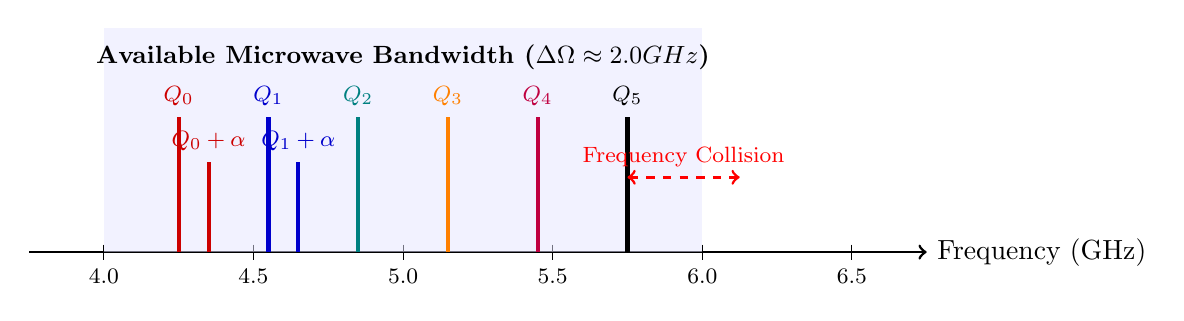
\begin{tikzpicture}[scale=0.95]
        % Axis
        \draw[->, line width=1pt] (0,0) -- (12,0) node[right] {Frequency (GHz)};
        \foreach \x/\label in {1/4.0, 3/4.5, 5/5.0, 7/5.5, 9/6.0, 11/6.5}
            \draw (\x,0.1) -- (\x,-0.1) node[below] {\footnotesize \label};
            
        % Bandwidth region
        \fill[blue!10, opacity=0.5] (1,0) rectangle (9,3);
        \node at (5,2.6) {\small\textbf{Available Microwave Bandwidth ($\Delta\Omega \approx 2.0\text{ GHz}$)}};
        
        % Qubit peaks
        \draw[line width=1.5pt, red!80!black] (2,0) -- (2,1.8) node[above] {\footnotesize $Q_0$};
        \draw[line width=1.5pt, red!80!black] (2.4,0) -- (2.4,1.2) node[above] {\footnotesize $Q_0 + \alpha$};
        \draw[line width=1.5pt, blue!80!black] (3.2,0) -- (3.2,1.8) node[above] {\footnotesize $Q_1$};
        \draw[line width=1.5pt, blue!80!black] (3.6,0) -- (3.6,1.2) node[above] {\footnotesize $Q_1 + \alpha$};
        \draw[line width=1.5pt, teal] (4.4,0) -- (4.4,1.8) node[above] {\footnotesize $Q_2$};
        \draw[line width=1.5pt, orange] (5.6,0) -- (5.6,1.8) node[above] {\footnotesize $Q_3$};
        \draw[line width=1.5pt, purple] (6.8,0) -- (6.8,1.8) node[above] {\footnotesize $Q_4$};
        \draw[line width=1.5pt, black] (8.0,0) -- (8.0,1.8) node[above] {\footnotesize $Q_5$};
        
        % Collision overlap warning
        \draw[<->, line width=1pt, dashed, red] (8.0, 1.0) -- (9.5, 1.0) node[midway, above] {\footnotesize Frequency Collision};
    \end{tikzpicture}
    \caption{The frequency crowding problem in monolithic planar transmons. As the number of qubits on a single chip increases, the finite 2.0 GHz amplifier band becomes saturated with fundamental frequencies and leakage energy levels ($\omega_{01} + \alpha$).}
    \label{fig:frequency_crowding}
\end{figure}

In a monolithic chip, each transmon added to the lattice introduces an additional fundamental frequency and non-linear transitions. Because modern electron-beam lithography has an intrinsic fabrication tolerance dispersion in Josephson junction area ($\Delta A_J / A_J \approx 2\text{ to }5\%$), junction critical currents $I_c$ vary stochastically:

\begin{equation}
    \omega_{01} \propto \sqrt{I_c} \propto A_J^{1/4}
\end{equation}

This fabrication imprecision causes random frequency collisions. On a 100-qubit monolithic chip, the probability of at least one pair of nearest-neighbor qubits suffering an unresolvable frequency collision exceeds 90\%, causing irreversible gate fidelity decay ($F < 0.99$).

---

\section{Silicon Fabrication Yield and Defect Economics}

A third insurmountable challenge to monolithic scalability is \textbf{semiconductor die yield}. In classical silicon semiconductor manufacturing, the yield $Y$ of a chip of area $A$ with defect density $D$ is governed by the Murphy or Poisson yield model:

\begin{equation}
    Y = e^{-A \cdot D} \quad \text{or} \quad Y = \left( \frac{1 - e^{-A \cdot D}}{A \cdot D} \right)^2
\end{equation}

In classical microprocessors, a defect in an L3 cache line can be mitigated through laser cutting and redundant cache rows. In a monolithic quantum processor executing topological error correction codes (e.g., surface codes on a square or rotated lattice), \textbf{every single qubit must function with gate fidelities above the fault-tolerance threshold} ($F_{\text{gate}} > 99.0\%$).

A single broken Josephson junction, an open-circuit flux line, or a two-level system (TLS) defect in the substrate silicon dielectric creates a "dead qubit" that creates a puncture in the surface code, exponentially increasing the logical error rate $\Lambda_L$:

\begin{equation}
    P_{\text{chip\_success}} = \prod_{k=1}^{N} p_{\text{qubit\_operational}}(k) = (p_{\text{good}})^N
\end{equation}

Even if the per-qubit operational probability is an astonishingly high $p_{\text{good}} = 0.999$ (99.9\%):
\begin{itemize}
    \item For $N = 100$ qubits: $P_{\text{success}} = (0.999)^{100} \approx 90.4\%$
    \item For $N = 1,000$ qubits: $P_{\text{success}} = (0.999)^{1,000} \approx 36.7\%$
    \item For $N = 10,000$ qubits: $P_{\text{success}} = (0.999)^{10,000} \approx 0.000045\%$
    \item For $N = 1,000,000$ qubits: $P_{\text{success}} \to 0.00000000000000\%$
\end{itemize}

Building a monolithic quantum processor containing one million defect-free qubits on a single wafer is an economic and fabrication impossibility. 

\begin{definitionbox}{The Modular Chiplet Solution}
Rather than attempting to manufacture an impossible $10^6$-qubit monolithic wafer with zero yield, scalable engineering dictates manufacturing modular \textbf{Quantum Processing Units (QPUs)} containing 50 to 100 high-yield, pristine qubits, and interconnecting these modular chiplets using quantum entanglement networks.
\end{definitionbox}

---

\section{The Architectural Paradigm Shift: The Multi-QPU Execution Model}

To bypass the cryogenic wiring wall, the frequency crowding wall, and the die yield wall, the quantum computing industry is converging on the **Distributed Multi-QPU Architecture**.

\begin{table}[htbp]
\centering
\small
\begin{tabularx}{\textwidth}{l X X X}
\toprule
\textbf{Company / Vendor} & \textbf{Physical Modality} & \textbf{Inter-QPU Network Architecture} & \textbf{Target Topology} \\
\midrule
\textbf{IBM Quantum} & Superconducting Transmons & Metre-long cryogenic coaxial cables (Flamingo architecture) & Modular cryostats, planar coupling \\
\addlinespace
\textbf{IonQ} & Trapped $^{171}\text{Yb}^+$ Ions & Photonic interconnects with optical cavity phase switches & Reconfigurable optical crossbar \\
\addlinespace
\textbf{Atom Computing} & Neutral $^{87}\text{Sr}$ Atoms & Optical tweezer shuttling across vacuum cells & Multi-cell optical array \\
\addlinespace
\textbf{PsiQuantum} & Silicon Photonics & Integrated optical fiber delay lines and waveguide switches & Distributed photonic datacenter \\
\bottomrule
\end{tabularx}
\caption{Industry roadmaps converging toward distributed multi-QPU execution.}
\label{tab:industry_roadmaps}
\end{table}

In this modular architecture, computation is distributed across physical nodes:
\begin{itemize}
    \item \textbf{Intra-QPU Gates:} Two-qubit gates between qubits residing on the same chip execute via high-speed, local capacitive couplers (latencies $\sim 20-50\text{ ns}$).
    \item \textbf{Inter-QPU Gates:} Gates between qubits residing on physically separated chips cannot execute via physical couplers. They \textbf{must} execute via entanglement-assisted communication channels: \textbf{Quantum Gate Teleportation}.
\end{itemize}

---

\section{Chapter Summary and Compiler Implications}
This chapter has demonstrated that physical hardware limits enforce an absolute ceiling on monolithic quantum computing. Scaling beyond thousands of qubits requires modular quantum processing units connected by quantum networks.

However, moving from a monolithic architecture to a distributed multi-QPU architecture transfers the primary burden of complexity \textbf{from the hardware engineer to the compiler architect}:
\begin{enumerate}
    \item The compiler must partition logical algorithms across heterogeneous nodes to minimize cross-chip interactions.
    \item The compiler must automatically synthesize quantum gate teleportation protocols (EPR generation, Bell measurements, classical feedforward) for all non-local gates.
    \item The compiler must schedule entanglement generation to mask network latency and prevent decoherence.
\end{enumerate}

Solving these three problems is the sole focus of the remainder of this book. In Chapter~\ref{ch:hardware_interconnects}, we examine the physical interconnect technologies that make inter-QPU entanglement possible.
